
\chapter{Proof of Lemma~3.4.5} %\ref{lem:ZZ0}}
\label{sec:proof_pdreeb}

In this proof, we use the notations of Definition~\ref{def:Morse-type}.
Let $$0<\epsilon<\frac{1}{2}\min_{k=1,...,n}\ \min\{s_k-a_k,a_k-s_{k-1}\}.$$ %(a_{k+1}-a_k)$.
The idea of the proof is to replace the right inverse of the
projection $\pi:X\to\Reeb_f(X)$ by a continuous map
$\sigma:\Reeb_f(X)\to X$ such that the composition $\pi\circ\sigma$ is
homotopic to the identity of $\Reeb_f(X)$. In order to make our new
$\sigma$ compatible with the function~$f$, we need to perturb $f$ to
some other function $g$ whose
preimages of intervals $[s_i,s_j]$, $i\leq j$, 
are equal to the ones of $f$.

Let $g:X\rightarrow\R$ be defined by:
$$\forall x\in X,\ g(x)=\left\{ \begin{array}{l} f(x)\text{   if }\displaystyle\min_{k=1,...,n} |f(x)-a_k|>2\epsilon \\
						a_i\text{   otherwise, where }i=\text{argmin}_k|f(x)-a_k| \end{array} \right.$$

As $g$ is constant on equivalence classes of $\sim_f$,  there is an induced map $\tilde{g}:\Reeb_f(X)\rightarrow\R$.
Moreover, for any $i\leq j$, we have $g^{-1}([s_i,s_j])=f^{-1}([s_i,s_j])$ by definition of $g$ and $\epsilon$. The
same holds for $\tilde f$ and $\tilde g$.

%%%
\begin{figure}[htb]
\begin{center}
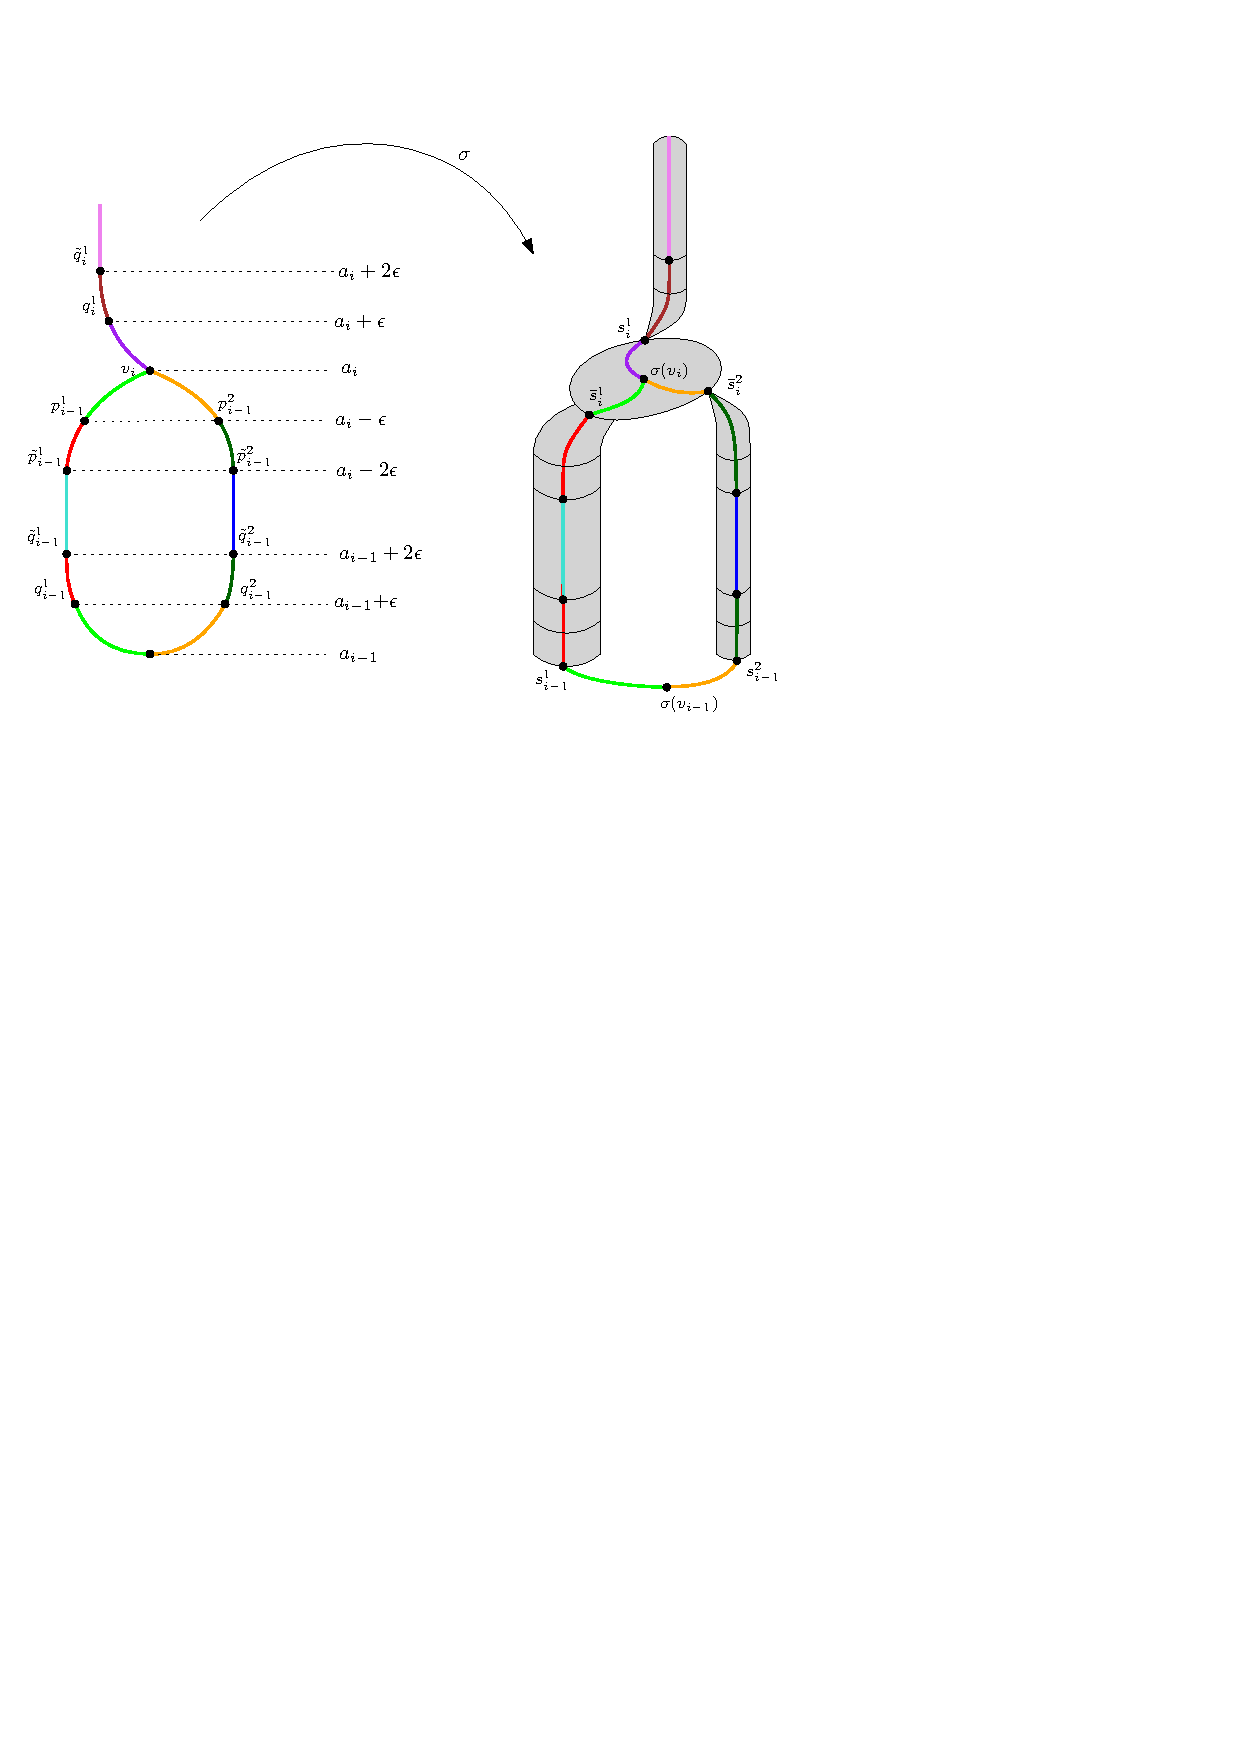
\includegraphics[width=13cm]{figures/Sections}
\caption[Images of paths in Reeb graph]{\label{fig:contsect}
The left panel displays the Reeb graph and the right panel displays
the space~$X$ itself.
$\sigma$ sends an arc of the Reeb graph to the path with the same color in $X$. }
\end{center}
\end{figure}

Now we want to define a continuous map $\sigma:\Reeb_f(X)\rightarrow X$ 
such that the composition with the projection $\pi\circ\sigma$ is homotopic to $\text{id}_{\Reeb_f(X)}$.
For any node $v_i$, if $Y_{i-1}$ has $k_i$ connected components $Y_{i-1}^1,...,Y_{i-1}^{k_i}$ and 
$Y_i$ has $l_i$ connected components $Y_i^1,...,Y_i^{l_i}$, we let $\{(\tilde{p}_{i-1}^k,p_{i-1}^k)\ |\ k=1,...,k_i\}$ 
and $\{(q_i^l,\tilde{q}_i^l)\ |\ l=1,...,l_i\}$ denote points in $\Reeb_f(X)$ located at levelsets 
$a_i-2\epsilon,a_i-\epsilon,a_i+\epsilon,a_i+2\epsilon$.
See Figure~\ref{fig:contsect}.
For any $i=1,...,n$ and any $l=1,...,l_i$,
we select an arbitrary point $y_i^l\in Y_i^l$
and we let $s_i^l=\phi_i(y_i^l,a_i)$
and $\bar{s}_{i+1}^l=\psi_i(y_i^l,a_{i+1})$. \\

For any critical value $a_i$ and any vertex $v_i$ of $\Reeb_f(X)$ at that
level, we let $\sigma(v_i)$ be an arbitrary point in $\pi^{-1}(v_i)$,
$\sigma(q_i^l)=s_i^l$, and $\sigma(p_{i-1}^k)=\bar{s}_{i}^k$.
Moreover, as there exists a path
$\gamma_k^{i,-}:[a_i-\epsilon,a_i]\rightarrow X$ from $\bar{s}_{i}^k$ to
$\sigma(v_i)$, $\sigma$ sends the arc $[p_{i-1}^k,v_i]$ to this path
$\gamma_{k}^{i,-}$.  Similarly, it sends the arc $[v_i,q_i^l]$ to a path
$\gamma_l^{i,+}:[a_i,a_i+\epsilon]\rightarrow X$ from $\sigma(v_i)$ to
$s_i^l$.  Finally, $\sigma$ also monotonically reparametrizes the
arcs $[\tilde{p}_i^k,p_i^k]$ and $[q_i^l,\tilde{q}_i^l]$.  Let
$\text{param}_i^+:[a_i+\epsilon,a_i+2\epsilon]\rightarrow[a_i,a_i+2\epsilon]$,
and
$\text{param}_i^-:[a_i-2\epsilon,a_i-\epsilon]\rightarrow[a_i-2\epsilon,a_i]$
be these reparametrizations. Again, see Figure~\ref{fig:contsect}. 
More formally, let $x\in X$ and assume that $a_i\leq f(x)\leq a_{i+1}$
and that $\pi(x)$ belongs to the $l$-th edge of the Reeb graph between
these two critical values. Then:
%,
%$\text{param}_l^+:[a_i,a_i+\epsilon]\rightarrow[0,1]$ and
%$\text{param}_l^-:[a_{i+1}-\epsilon,a_{i+1}]\rightarrow[0,1]$
%be the linear re-parametrizations induced by $\sigma$. Then: \\

\begin{itemize}
\item $\sigma\circ\pi(x)=\mu_i(y_i^l,f(x))$ if $a_i+2\epsilon\leq f(x)\leq a_{i+1}-2\epsilon$;

\item $\sigma\circ\pi(x)=\mu_i(y_i^l,\text{param}_i^+\circ f(x))$ if $a_i+\epsilon\leq f(x)\leq a_i+2\epsilon$;

\item $\sigma\circ\pi(x)=\mu_i(y_i^l,\text{param}_{i+1}^-\circ f(x))$ if $a_{i+1}-2\epsilon\leq f(x)\leq a_{i+1}-\epsilon$;

\item $\sigma\circ\pi(x)=\gamma_l^{i,+}(f(x))$ if $a_i\leq f(x)\leq a_i+\epsilon$;

\item $\sigma\circ\pi(x)=\gamma_l^{i+1,-}(f(x))$ if $a_{i+1}-\epsilon\leq f(x)\leq a_{i+1}$.
\end{itemize}


By construction we have $g\circ\sigma=\tilde{g}$ and $\tilde{g}\circ\pi=g$ (note that this is not true for $f$). 

Let $i\leq j$ and $I=[s_i,s_j]$.
Then we have $\pi(g^{-1}(I))\subseteq \tilde g^{-1} (I)$. 
Hence, $\pi$ induces a morphism between $H_0(g^{-1}(I))$ and $H_0(\tilde g^{-1}(I))$. 
Let us show that this morphism is an isomorphism. Since $\pi$ is surjective, this boils down to
showing that $x,y$ are connected in $g^{-1}(I)$ if and only if $\pi(x),\pi(y)$ are connected in $\tilde g^{-1}(I)$.
%
\begin{itemize}
\item If $x,y$ are connected in $g^{-1}(I)$, then so are $\pi(x),\pi(y)$ in $\tilde g^{-1}(I)$, by
  continuity of $\pi$ and the fact that $\tilde{g}\circ\pi=g$.
%
\item If $\pi(x),\pi(y)$ are connected in $\tilde g^{-1}(I)$, then choose a path $\gamma$
  connecting $\pi(x)$ and $\pi(y)$. Now by definition of $\sigma$,
  there exists a path $\gamma_x$ connecting $x$ and
  $\sigma\circ\pi(x)$ in $g^{-1}(I)$.  Indeed, $\sigma$ can send
  $\pi(x)$ to five different locations in $g^{-1}(I)$
  according to the value of $f(x)$, as seen above.  
  Assume $f(x)\notin \Crit(f)$. Since there is a path $\tilde \gamma$ between
  $x$ and $\mu_i(y_i^l,f(x))$, one can always find a path $\gamma_x$
  between $x$ and $\sigma\circ\pi(x)$ in $g^{-1}(I)$ with an
  appropriate combination of $\tilde \gamma$, $\mu_i(y_i^l,\cdot)$ and
  $\gamma_l^{(i,+)/(i+1,-)}$.  
  Now, assume $f(x)\in\Crit(f)$, and let $v_i=\pi(x)$. Then $\sigma(v_i)$ and $x$
  both belong to $\pi^{-1}(v_i)$, so they belong to the same connected component of 
  the $g^{-1}(g(x))$ and one can find a path between them in $g^{-1}(I)$.
  Similarly, there exists a path $\gamma_y$
  connecting $\sigma\circ\pi(y)$ and $y$ in $g^{-1}(I)$. Then
  $\gamma_y\circ\sigma(\gamma)\circ\gamma_x$ is a path
  between $x$ and $y$ in $g^{-1}(I)$
  by continuity of $\sigma$ and the fact that $g\circ\sigma=\tilde{g}$.
  So $x,y$ are connected in $g^{-1}(I)$.
\end{itemize}
%
Since $g^{-1}(I)=f^{-1}(I)$ and $\tilde g^{-1}(I)= \tilde f^{-1}(I)$, we have that 
$\pi_*$ is an isomorphism between $H_0(f^{-1}(I))$ and $H_0(\tilde f^{-1}(I))$, and the proof is complete. 

\begin{comment}
%%%%%%%%%%%%%%%%%
\section{Proof of Lemma~\ref{lem:dfdmerge}}
\label{sec:proof_dfd}

This proof uses the same construction as the proof of Proposition~3.1 in~\cite{Carriere17a}.

We first prove the result with the stronger assumption that critical values of $\Reeb_g$
are all located inside the interiors of the intervals of $S$, that is $\Crit(\Reeb_g)\subseteq \bigcup_{I\in S} {\rm int}\ I$.
We define explicit continuous maps $\phi:\Reeb_g\rightarrow\Reeb_{g'}$ and
$\psi:\Reeb_{g'}\rightarrow\Reeb_g$ as depicted in
Figure~\ref{fig:fdmerge}.  More precisely, since all critical values of $\Reeb_g$ belong
to $\bigcup_{I\in S} {\rm int}\ I$, we only need to specify $\phi$ and $\psi$
inside each interval $I\in S$ and then ensure that the piecewise-defined maps are assembled consistently.
Let $I=[a,b]$ be such an interval. Since $a,b\not\in \Crit(g)$, there exist two levels 
$a < \alpha\leq\beta < b$ such that $\Reeb_g$ is only composed of arcs in
$[a,\alpha]$ and $[\beta,b]$ (dashed lines in Figure~\ref{fig:fdmerge}).  
For any connected component~$C$ of $g^{-1}([a,b])$, the map $\phi$ sends all points of
$C\cap g^{-1}([\alpha,\beta])$ to the corresponding critical
point $y_C\in\Reeb_{g'}$ created by $\Merge_{a,b}$, and it extends the
arcs of $C\cap g^{-1}([a,\alpha])$ (resp. $C\cap g^{-1}([\beta,b])$) 
into arcs of $(g')^{-1}([a,\bar a])$ (resp. $(g')^{-1}([\bar a,b])$). 
In return, the map $\psi$ sends the critical
point~$y_C$ to an arbitrary point of $C$.  Then, since the Merge
operation preserves connected components, for each arc $A'$ of
$(g')^{-1}([a,b])$ connected to~$y_C$, there is at
least one corresponding path $A$ in $\Reeb$ whose endpoint in
$g^{-1}(a)$ or $g^{-1}(b)$ matches with the one of $A'$
(see the colors in Figure~\ref{fig:fdmerge}).  Hence $\psi$ sends
$A'$ to $A$ and the piecewise-defined maps
are assembled consistently.

\begin{figure}[htb]\centering
\includegraphics[width=10cm]{figures/fdmerge}
\caption{\label{fig:fdmerge}
The effects of $\phi$ and $\psi$ around a specific critical value $a_i$ of $f$. Segments are matched according
to their colors (up to reparameterization).
}
\end{figure}

\noindent Let us bound the
three terms in the $\max\{\cdots\}$ in~(\ref{eq:dfd})
with this choice of maps $\phi, \psi$: 
\begin{itemize}

\item We first  bound $\|g'-g\circ\psi\|_\infty$. Let $x\in\Reeb_{g'}$. Either $g'(x)\not\in \bigcup_{I\in S} I$,  
and in this case we have $g'(x)=g(\psi(x))$ by definition of~$\psi$;
or, there is $I=[a,b]\in S$ such that $g'(x)\in \mathring{I}$ and then $g(\psi(x))\in [a,b]$.
In both cases $|g'(x)-g\circ\psi(x)| < b-a$. Hence, $\|g'-g\circ\psi\|_\infty < \max_{I\in S}|I|$.

\item Since the previous proof is symmetric in $g$ and $g'$, one also has $\|g-g'\circ\phi\|_\infty < \max_{I\in S}|I|$.

\item We now bound $D(\phi,\psi)$: 

Let $(x,\phi(x)),(\psi(y),y)\in C(\phi,\psi)$ (the cases $(x,\phi(x)),(x',\phi(x'))$
and $(\psi(y),y),(\psi(y'),y')$ are similar). Let $\pi_{g'}:[0,1]\rightarrow\Reeb_{g'}$ be a continuous path from $\phi(x)$ to $y$  
which achieves $d_{g'}(\phi(x),y)$.

\begin{itemize}

\item Assume $g(x)\not\in \bigcup_{I\in S} I$. Then one has $\psi\circ\phi(x)=x$.
Hence, $\pi_g:=\psi\circ\pi_{g'}$ is a path from $x$ to $\psi(y)$. Moreover, since $\|g'-g\circ\psi\|_\infty < b-a$,
it follows that
\begin{equation}\label{eqs:noname}
\begin{array}{l}\max\ \im(g\circ \pi_g) < \max\ \im(g'\circ \pi_{g'}) + \max_{I\in S}|I|,\\[0.5ex]
\min\ \im(g\circ\pi_g) > \min\ \im(g'\circ\pi_{g'}) - \max_{I\in S}|I|.\end{array}
\end{equation}
Hence, one has 
$$\begin{array}{l}d_g(x,\psi(y))\leq \max\ \im(g\circ\pi_g)-\min\ \im(g\circ\pi_g) < d_{g'}(\phi(x),y) + 2\max_{I\in S}|I|,\\
-d_g(x,\psi(y))\geq \min\ \im(g\circ\pi_g)-\max\ \im(g\circ\pi_g) > -d_{g'}(\phi(x),y)- 2\max_{I\in S}|I|.\end{array}$$
This shows that $|d_g(x,\psi(y))-d_{g'}(\phi(x),y)| < 2\max_{I\in S}|I|$.

\item Assume that there is $I=[a,b]\in S$ such that $g(x)\in (a,b)$.
Then, by definition of $\phi,\psi$, we have  $g'(\phi(x))\in(a,b)$, 
and, since $\phi$ and $\psi$ preserve connected components, there is a path
$\pi'_g:[0,1]\rightarrow\Reeb_g$ from $x$ to $\psi\circ\phi(x)$
within the interval $[a,b]$, which itself is
included in the interior of the offset ${\rm im}(g'\circ\pi_{g'})^{b-a}$. Let now
$\pi_g$ be the concatenation of $\pi'_g$ with $\psi\circ\pi_{g'}$, which goes from $x$ to
$\psi(y)$.
Since $\|g'-g\circ\psi\|<\max_{I\in S}|I|$, it follows that ${\rm im}(g\circ\psi\circ\pi_{g'})\subseteq{\rm int}\ {\rm im}(g'\circ\pi_{g'})^{\max_{I\in S}|I|}$, 
and since ${\rm im}(g\circ\pi_g)={\rm im}(g\circ\pi'_g)\cup{\rm im}(g\circ\psi\circ\pi_{g'})$ by
concatenation, one finally has ${\rm im}(g\circ\pi_g)\subseteq {\rm int}\ {\rm im}(g'\circ\pi_{g'})^{\max_{I\in S}|I|}.$ Hence, the 
inequalities of~(\ref{eqs:noname}) hold, implying that $|d_g(x,\psi(y))-d_{g'}(\phi(x),y)| < 2\max_{I\in S}|I|$.
\end{itemize} 
Since these inequalities hold for any couples $(x,\phi(x))$ and $(\psi(y),y)$, we deduce that $D(\phi,\psi) \leq 2\max_{I\in S}|I|$.
\end{itemize}

In the general case where an endpoint of an interval of $S$ can be a critical value of $g$, 
one needs to slightly change the definition of $\phi$. More precisely, $\alpha$ and $\beta$
have to be taken outside but arbitrarily close to $[a,b]$. Then, the previous proof extends verbatim. 
\end{comment}